\section{Giới thiệu đề tài}

\subsection{Bối cảnh và vấn đề đặt ra}
Trong lĩnh vực trò chơi điện tử chiến thuật theo lượt, cờ vua truyền thống từ lâu đã được xem là chuẩn mực kinh điển về chiều sâu tư duy logic và tính cân bằng. Tuy nhiên, đối với nhóm người chơi hiện đại, cờ vua cổ điển tồn tại hai rào cản đáng kể: (i) thời lượng ván đấu kéo dài với nhiều khai cuộc mang tính học thuộc, làm giảm yếu tố bất ngờ; và (ii) cấu trúc luật cố định, thiếu các cơ chế tùy biến đội hình trước trận hoặc nâng cấp sức mạnh quân cờ trong trận như các trò chơi chiến thuật hiện đại.

Ở chiều ngược lại, các biến thể cờ chiến thuật mới nổi thường thiên về yếu tố may rủi hoặc đồ họa bắt mắt mà ít chú trọng đến thiết kế kiến trúc tách biệt giữa luật chơi và phần hiển thị. Điều này gây khó khăn khi vừa cần vận hành mượt mà ở chế độ nhiều người chơi trực tuyến (Online Multiplayer), vừa cần mô phỏng tốc độ cao để huấn luyện Trí tuệ nhân tạo (AI). Bên cạnh đó, nhu cầu cá nhân hóa danh tính người chơi trong không gian 3D (như tạo hình đại diện từ ảnh chân dung thực tế) ngày càng được quan tâm nhưng vẫn còn nhiều thách thức về thời gian xử lý, độ chính xác hình học khuôn mặt 3D và xử lý ánh sáng bề mặt da.

Xuất phát từ các nhận định trên, nhóm thực hiện đề tài \textbf{Phát triển game ``Convergence Chess''} -- một trò chơi cờ chiến thuật 3D trên nền tảng Unity 6 \cite{unity6}, kết hợp cấu trúc di chuyển của cờ vua với cơ chế kinh tế điểm hành động tích lũy (AP), vật cản sinh ngẫu nhiên và đặc biệt là cơ chế \textbf{hợp thể quân cờ} kèm trạng thái đòn bồi (\textbf{Surge}). Dự án đồng thời xây dựng hai hướng tác nhân AI chính là \textbf{Hybrid Bot} (kết hợp tìm kiếm Minimax, học tăng cường PPO \cite{mlagents} và mạng đánh giá nhanh NNUE \cite{nnue}) và \textbf{LLM Bot} (tiến hóa luật đánh giá bằng Mô hình Ngôn ngữ Lớn theo hướng FunSearch \cite{funsearch}), tích hợp chế độ đối kháng trực tuyến qua Photon Fusion 2 \cite{photon_fusion} cùng phân hệ mở rộng tùy biến nhân vật 3D từ ảnh chân dung (Smart Customization).

\subsection{Tổng quan luật chơi và cơ chế cốt lõi của Convergence Chess}
Khác với bàn cờ $8 \times 8$ truyền thống, \textit{Convergence Chess} được thiết kế tinh gọn trên bàn cờ $6 \times 6$ nhằm đẩy nhanh nhịp độ giao tranh và tăng mật độ tính toán chiến thuật trong từng lượt đi (minh họa không gian chiến thuật và tạo hình quân cờ tại Hình \ref{fig:intro_concept}).

\begin{figure}[H]
    \centering
    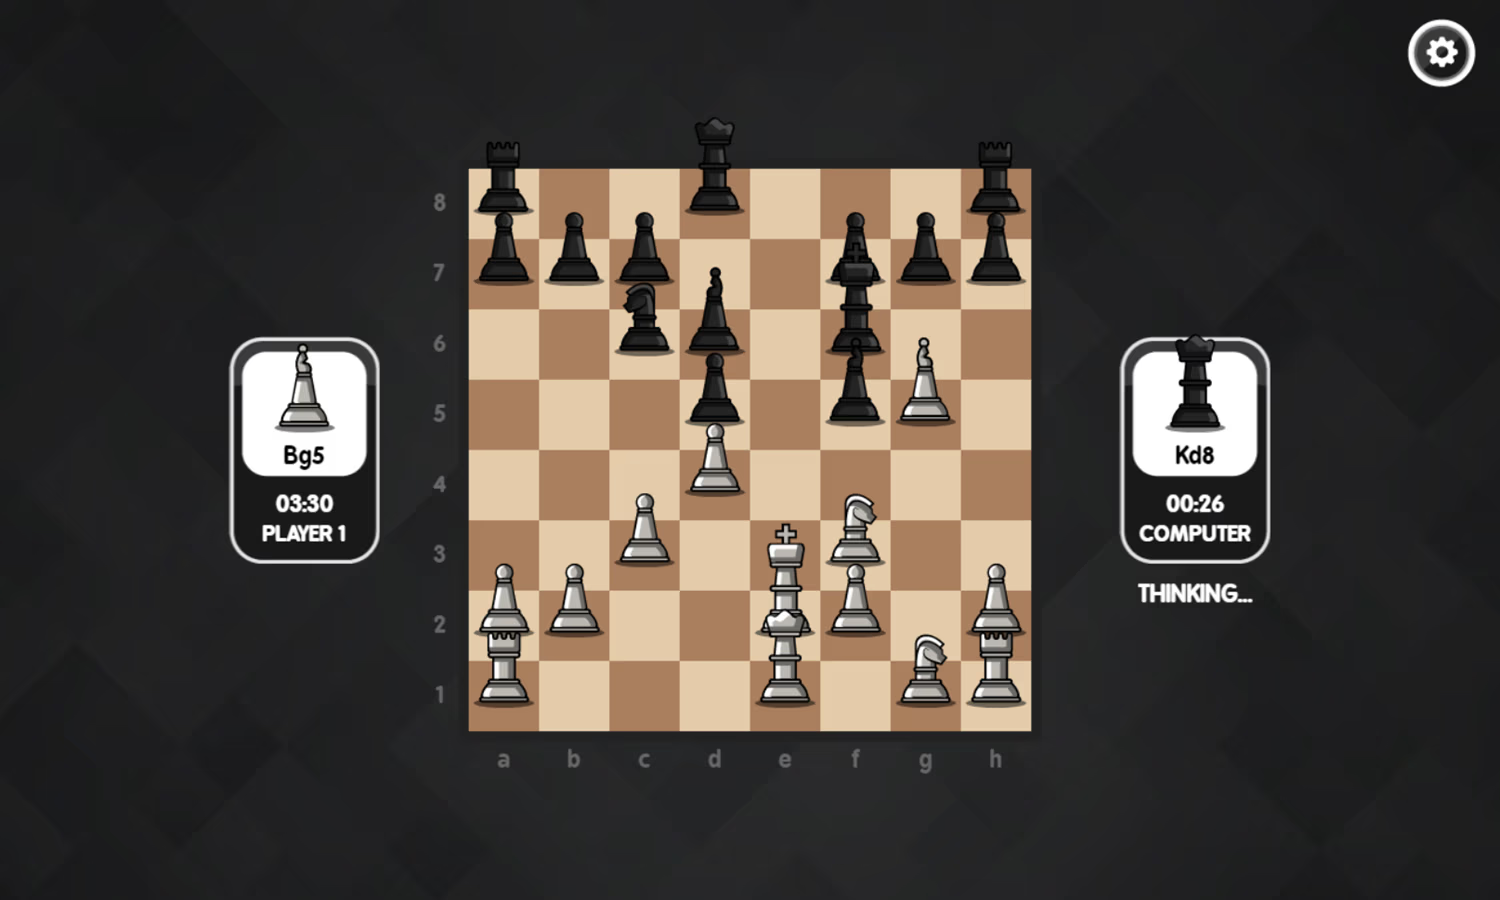
\includegraphics[width=0.68\textwidth]{Content/Giới thiệu/images/chess.png}
    \caption{Minh họa ý tưởng không gian chiến thuật và tạo hình quân cờ của Convergence Chess}
    \label{fig:intro_concept}
\end{figure}

\subsubsection{Không gian bàn cờ, đội hình và vật cản ngẫu nhiên}
Bàn cờ gồm $36$ ô được đánh chỉ số từ $0$ đến $35$ theo công thức $\text{chỉ số} = y \times 6 + x$:
\begin{itemize}
    \item \textbf{Sân nhà Người chơi 1:} Hàng 0 và hàng 1 (từ ô $0$ đến ô $11$), quân Vua đứng cố định tại ô $(3,0)$ (tương ứng ô d1).
    \item \textbf{Sân nhà Người chơi 2:} Hàng 4 và hàng 5 (từ ô $24$ đến ô $35$), quân Vua đứng cố định tại ô $(3,5)$ (tương ứng ô d6).
    \item \textbf{Vùng trung tuyến:} Hàng 2 và hàng 3 (từ ô $12$ đến ô $23$). Khi khởi tạo ván đấu, hệ thống sinh ngẫu nhiên $1$ đến $2$ ô vật cản chỉ trong vùng trung tuyến này dựa trên một hạt giống ngẫu nhiên xác định. Các quân di chuyển theo đường trượt (Xe, Tượng, Hậu) bị chặn đường bởi vật cản, trong khi quân có kỹ năng nhảy chữ L (Mã) được phép nhảy vượt qua.
    \item \textbf{Thiết lập đội hình trước trận:} Trước khi vào trận, mỗi người chơi có ngân sách hiện hành là \textbf{12 điểm đội hình} để mua và tự do sắp xếp quân cờ trong sân nhà của mình ngoài quân Vua mặc định (chi tiết chi phí và kỹ năng từng loại quân được tổng hợp tại Bảng \ref{tab:piece_roster}).
\end{itemize}

\begin{table}[H]
    \centering
    \caption{Bảng chi phí điểm đội hình, kỹ năng di chuyển gốc và kỹ năng thức tỉnh khi hợp thể}
    \label{tab:piece_roster}
    \begin{tabularx}{\textwidth}{L{2.2cm} C{1.6cm} L{2.8cm} L{2.7cm} Y}
        \toprule
        \textbf{Quân cờ} & \textbf{Chi phí (điểm)} & \textbf{Chi phí AP di chuyển} & \textbf{Kỹ năng di chuyển gốc} & \textbf{Kỹ năng thức tỉnh khi làm quân nguồn hợp thể} \\
        \midrule
        Tốt & 1 & 1 AP mỗi bước tiến hoặc ăn chéo & Không có & Cộng thêm AP: tự động hồi thêm $+1$ AP ở đầu mỗi lượt chơi. \\
        Mã & 3 & 2 AP cố định mỗi nước nhảy & Nhảy chữ L vượt vật cản và quân chắn & Phá khiên: xuyên thủng và phá hủy trực tiếp lớp khiên hộ mệnh. \\
        Tượng & 4 & 1 AP mỗi ô trượt chéo & Trượt tự do theo 4 đường chéo & Hút năng lượng chiến đấu: hoàn trả $+1$ AP ngay khi tiêu diệt 1 quân địch. \\
        Xe & 5 & 1 AP mỗi ô trượt ngang/dọc & Trượt tự do theo hàng ngang và cột dọc & Khiên hộ mệnh: tạo 1 lớp khiên chặn đòn tiêu diệt đầu tiên và đẩy lùi kẻ tấn công. \\
        Hậu & 6 (khóa mua trước trận) & 1 AP mỗi ô trượt 8 hướng & Trượt tự do theo cả 8 hướng & Rút điểm hành động: trừ $-1$ AP của đối thủ khi tiêu diệt 1 quân địch. Hiện chỉ đạt được thông qua phong cấp Tốt trong trận. \\
        Vua & Cố định & 1 AP (di chuyển 1 ô theo 8 hướng) & Không có & Không được phép tham gia hợp thể; mất Vua là thua trận. \\
        \bottomrule
    \end{tabularx}
\end{table}

\subsubsection{Kinh tế điểm hành động (AP) và cơ chế chống kéo dài trận đấu}
Thay vì cho phép mọi quân cờ di chuyển miễn phí với cự ly bất kỳ như cờ vua cổ điển, mỗi hành động trong \textit{Convergence Chess} đều tiêu hao Điểm hành động (AP) theo quy tắc cân bằng linh hoạt:
\begin{itemize}
    \item Hai bên khởi đầu với lượng AP bằng nhau ($3$ AP). Ở đầu mỗi lượt, người chơi được hồi $+2$ AP (cộng thêm $+1$ AP cho mỗi quân đang sở hữu kỹ năng cộng thêm AP), tích lũy tối đa đến ngưỡng \textbf{5 AP} và không bao giờ giảm xuống dưới $0$.
    \item Người chơi có quyền chủ động bỏ lượt để tích lũy AP cho các nước đi tầm xa hoặc hợp thể ở lượt sau, nhưng bị giới hạn tối đa $3$ lần bỏ lượt mỗi trận nhằm ngăn chặn hành vi câu giờ. Nếu tới lượt một phe không còn bất kỳ hành động hợp lệ nào (đã hết lượt bỏ lượt và không có nước đi đủ AP), hệ thống sẽ xử thua cho phe đó.
    \item Toàn bộ ván đấu bị giới hạn tối đa $60$ lượt đi lẻ; nếu đạt đến giới hạn này mà chưa có bên nào tiêu diệt được Vua đối phương, ván đấu được xử hòa.
\end{itemize}

\subsubsection{Cơ chế hợp thể quân cờ, khiên hộ mệnh và đòn bồi Surge}
Điểm sáng tạo cốt lõi tạo nên tên gọi \textit{Convergence Chess} là hệ thống hợp thể quân cờ:
\begin{enumerate}
    \item \textbf{Điều kiện và chi phí hợp thể:} Một quân đồng minh A (quân nguồn, không phải Vua) di chuyển hợp lệ vào ô của quân đồng minh B (quân đích, không phải Vua) sẽ tiêu tốn tổng AP bằng chi phí di chuyển cộng với phụ phí hợp thể (hiện được thiết lập bằng $0$ để khuyến khích nhịp độ hợp thể sớm và có thể tinh chỉnh linh hoạt khi cân bằng trò chơi). Sau khi hợp thể, quân A rời khỏi bàn cờ; quân B giữ nguyên vị trí, kế thừa kỹ năng di chuyển gốc của A và đồng thời \textbf{thức tỉnh} kỹ năng đặc biệt của A. Để bảo đảm tính cân bằng, luật áp dụng hai giới hạn cứng: không cho phép hợp thể hai quân cùng loại cơ bản ban đầu và mỗi quân cờ chỉ được tham gia hợp thể tối đa một lần trong suốt ván đấu.
    \item \textbf{Cơ chế đòn bồi (Surge):} Ngay sau khi quân B hoàn tất hợp thể, nếu người chơi vẫn còn đủ AP cho ít nhất một nước đi hoặc đòn tấn công hợp lệ từ chính quân B, hệ thống sẽ mở giai đoạn \textbf{đòn bồi (Surge)} ngay trong lượt đó. Người chơi có thể chọn tung thêm một nước đi bồi bằng quân vừa hợp thể hoặc kết thúc lượt để giữ lại AP mà \textbf{không bị trừ} số lần bỏ lượt.
    \item \textbf{Tương tác giữa Khiên hộ mệnh và Phá khiên:} Khi một quân địch không có kỹ năng Phá khiên tấn công mục tiêu đang mang Khiên hộ mệnh, lớp khiên sẽ vỡ, mục tiêu sống sót tại chỗ còn kẻ tấn công bị đẩy ngược về ô xuất phát và vẫn mất AP. Ngược lại, kẻ tấn công có kỹ năng Phá khiên sẽ xuyên qua lớp khiên và tiêu diệt mục tiêu ngay lập tức.
    \item \textbf{Phong cấp Tốt:} Khi quân Tốt tiến tới hàng cuối cùng bên sân đối phương (hàng 5 với Người chơi 1, hàng 0 với Người chơi 2), quân này lập tức tiến hóa thành Hậu, nhận thêm kỹ năng trượt 8 hướng và kỹ năng rút AP đối thủ trong khi vẫn bảo lưu các kỹ năng sẵn có.
\end{enumerate}

\subsection{Mục tiêu và phạm vi thực hiện của giai đoạn 1 (DACN)}
Đề tài được triển khai xuyên suốt hai học kỳ gồm \textbf{Giai đoạn 1 -- Đồ án chuyên ngành (DACN)} và \textbf{Giai đoạn 2 -- Đồ án tốt nghiệp (DATN)}. Trong phạm vi \textbf{DACN (Giai đoạn 1)}, mục tiêu không phải phát hành ngay bản thương mại hoàn chỉnh, mà tập trung chứng minh tính khả thi kiến trúc, khảo sát công nghệ, xây dựng nguyên mẫu chơi thử thực tế và thu thập số liệu thực nghiệm làm nền tảng cho DATN:
\begin{itemize}
    \item \textbf{Kiến trúc phần mềm:} Xây dựng phần lõi xử lý luật chơi tách rời hoàn toàn khỏi đồ họa 3D, cho phép tái sử dụng nguyên vẹn trên cả 3 chế độ chơi (đấu với máy, đấu 2 người trên cùng máy, đấu trực tuyến) và chạy mô phỏng không hiển thị đồ họa ở tốc độ cao để phục vụ huấn luyện AI.
    \item \textbf{Khảo sát và thực nghiệm AI:} Tập trung xây dựng và đánh giá định lượng hai hướng tác nhân AI chủ lực là \textbf{Hybrid Bot} (phát triển qua chuỗi thành phần nền tảng gồm tìm kiếm Minimax Alpha-Beta, học bắt chước, học tăng cường PPO \cite{mlagents} và mạng đánh giá nhanh NNUE \cite{nnue}) và \textbf{LLM Bot} (tiến hóa hàm đánh giá biểu tượng bằng Mô hình Ngôn ngữ Lớn theo hướng FunSearch \cite{funsearch}).
    \item \textbf{Khảo sát và nguyên mẫu Multiplayer:} Đánh giá các giải pháp mạng, đo đạc thực nghiệm giữa cơ chế đồng bộ đối tượng (\texttt{Fusion Network Object}) và luồng dữ liệu tin cậy (\texttt{Fusion Reliable Data Stream}), hoàn thiện nguyên mẫu phòng chơi Lobby trên \texttt{GameMode.Shared} (tạo/vào phòng, chọn region, phân vai Trắng/Đen/Khán giả, đồng bộ đội hình và nước đi 4 bytes).
    \item \textbf{Khảo sát và nguyên mẫu tùy biến nhân vật 3D (Smart Customization):} Khảo sát các phương pháp tái tạo khuôn mặt 3D từ ảnh chân dung hiện có và tự xây dựng trọn vẹn quy trình sẵn sàng thương mại hóa (loại bỏ các mô hình phi thương mại), gồm nhánh tái tạo hình học khuôn mặt 25 thông số độc lập và nhánh xử lý bề mặt da, khử bóng đối xứng, vật liệu mắt cùng 6 kiểu tóc 3D tích hợp trực tiếp vào Unity 6.
    \item \textbf{Hoàn thiện bản chơi thử:} Kết nối toàn bộ luồng trải nghiệm từ màn hình chính, màn hình xây dựng đội hình, chọn chế độ chơi đến bàn cờ 3D $6 \times 6$ với bộ quân cờ phong cách Trung cổ, hoạt họa, hiệu ứng hình ảnh và âm thanh cơ bản.
\end{itemize}

Các hạng mục mang tính sản phẩm hóa và vận hành công khai như hệ thống đăng nhập tài khoản (Google/Facebook), lưu trữ đám mây, tự động ghép trận theo điểm xếp hạng Elo, hệ thống bạn bè, xử lý khôi phục kết nối nâng cao, hoàn thiện xử lý hết giờ/đầu hàng/cài đặt âm thanh và thử nghiệm người dùng quy mô lớn được quy hoạch rõ ràng sang \textbf{Giai đoạn 2 (DATN)}.

\subsection{So sánh với các sản phẩm tương tự và đánh giá ưu, nhược điểm của thiết kế lối chơi}
Bảng \ref{tab:market_comparison} đối chiếu \textit{Convergence Chess} với ba đại diện tiêu biểu trên thị trường nhằm làm rõ giá trị khác biệt của đề tài.

\begin{table}[H]
    \centering
    \caption{So sánh Convergence Chess với các trò chơi chiến thuật cờ tương tự}
    \label{tab:market_comparison}
    \begin{tabularx}{\textwidth}{L{2.8cm} Y Y Y Y}
        \toprule
        \textbf{Tiêu chí} & \textbf{Cờ vua truyền thống (Chess.com / Lichess)} & \textbf{Shotgun King / Pawnbarian} & \textbf{Teamfight Tactics} & \textbf{Convergence Chess} \\
        \midrule
        Kích thước và địa hình & Bàn $8 \times 8$ phẳng, cố định & Bàn $8 \times 8$ hoặc lưới nhỏ biến đổi theo màn & Bàn lưới lục giác, không vật cản địa hình & Bàn $6 \times 6$ kèm $1$--$2$ ô vật cản sinh ngẫu nhiên ở trung tuyến \\
        Cơ chế tài nguyên & Không có điểm hành động; mỗi lượt đi 1 quân & Tài nguyên đạn hoặc thẻ bài theo lượt & Kinh tế vàng mua tướng & Kinh tế điểm hành động tích lũy ($+2$/lượt, tối đa $5$), giới hạn số lần bỏ lượt \\
        Tùy biến đội hình và nâng cấp & Đội hình 16 quân cố định, chỉ phong Tốt & Nâng cấp ngẫu nhiên giữa các màn & Ghép 3 tướng giống nhau tăng cấp & Tự xây dựng đội hình (12 điểm) và hợp thể quân khác loại để thức tỉnh kỹ năng kèm đòn bồi Surge \\
        Chế độ chơi và AI & Đấu trực tuyến kèm máy đánh cờ Stockfish/Leela & Chủ yếu chơi đơn với máy & Đấu trực tuyến 8 người & Đấu với máy (Hybrid Bot và LLM Bot), đấu 2 người cùng máy và đấu trực tuyến \\
        Cá nhân hóa 3D & Bộ cờ 2D/3D có sẵn & Đồ họa điểm ảnh 2D & Linh thú bán sẵn & Thử nghiệm tạo nhân vật 3D từ ảnh chân dung (Smart Customization) \\
        \bottomrule
    \end{tabularx}
\end{table}

Bên cạnh giá trị khác biệt, thiết kế lối chơi của \textit{Convergence Chess} cũng đi kèm những ưu điểm và đánh đổi rõ rệt:
\begin{itemize}
    \item \textbf{Ưu điểm:} Bàn cờ $6 \times 6$ rút ngắn thời gian mỗi ván đấu và đẩy nhanh nhịp độ giao tranh ngay từ các lượt đầu; cơ chế tự chọn đội hình kết hợp hợp thể khác loại và đòn bồi Surge tạo ra không gian chiến thuật phong phú, hạn chế tình trạng học thuộc khai cuộc; vật cản sinh ngẫu nhiên ở trung tuyến giúp mỗi ván đấu mang tính biến hóa cao.
    \item \textbf{Nhược điểm và thách thức:} Nhiều cơ chế mới chồng lên nhau (kinh tế điểm hành động, $9$ kỹ năng nội tại gồm di chuyển và thức tỉnh, khóa hợp thể, đòn bồi Surge) tạo rào cản tiếp cận ban đầu cao hơn cờ vua truyền thống đối với người chơi mới; không gian $6 \times 6$ hẹp hơn nên dễ xảy ra tình trạng mất cân bằng lợi thế đi trước/đi sau nếu bộ tham số điểm hành động và chi phí đội hình chưa được hiệu chỉnh qua mô phỏng số lượng lớn.
\end{itemize}

\subsection{Phân công trách nhiệm trong nhóm thực hiện}
Dự án được thực hiện bởi 2 thành viên với ranh giới phân hệ rõ ràng, kết nối với nhau qua các giao diện trao đổi dữ liệu thống nhất:
\begin{itemize}
    \item \textbf{Thành viên 1 (Chủ trì Lõi luật chơi, AI và Smart Customization):} Thiết kế kiến trúc tổng thể tách biệt lõi và giao diện; xây dựng toàn bộ lõi luật chơi $6 \times 6$ (trạng thái bàn cờ, kiểm định nước đi, điều phối vòng lặp trận đấu và cấu hình cân bằng); xây dựng hai dòng tác nhân AI chính là \textbf{Hybrid Bot} (cùng chuỗi thành phần Minimax, học bắt chước, học tăng cường PPO, mạng đánh giá NNUE) và \textbf{LLM Bot}; phát triển quy trình tạo nhân vật 3D từ ảnh chân dung (Smart Customization) và cơ chế đồng bộ sự kiện hoạt họa quân cờ.
    \item \textbf{Thành viên 2 -- Đăng (Chủ trì Multiplayer và View Layer):} Khảo sát và hiện thực hệ thống Multiplayer trên nền tảng Photon Fusion (\texttt{OnlineSessionManager}, \texttt{OnlineDataBroadcastNetwork}, \texttt{NetworkController}, \texttt{PvPOnlModeBootstrapper}, đo benchmark mạng), chế độ PvP Offline (\texttt{BoardRotator}), tầng hiển thị bàn cờ và quân cờ 3D, toàn bộ hệ thống giao diện người dùng (màn hình chính, xây dựng đội hình, sảnh chờ trực tuyến, bảng thông số trong trận) và tích hợp hiệu ứng hình ảnh, âm thanh, bối cảnh 3D.
\end{itemize}
